% Source: graduate-coursework/Research/Intro_to_Agents/handouts/Part7_Parallelization.tex

\documentclass[border=4pt]{standalone}
\usepackage{amsmath,amssymb,amsfonts}
\usepackage[T1]{fontenc}
\usepackage{graphicx}
\usepackage{lmodern}
\usepackage{tikz}
\usepackage{xcolor}
\usetikzlibrary{shapes.geometric, arrows.meta, positioning, calc, fit, backgrounds, matrix, decorations.pathreplacing}

\definecolor{UofSCGarnet}{HTML}{73000a}
\definecolor{UofSCBlack}{HTML}{000000}
\definecolor{UofSCWhite}{HTML}{ffffff}
\definecolor{UofSCRose}{HTML}{CC2E40}
\definecolor{UofSCAtlantic}{HTML}{466A9F}
\definecolor{UofSCCongaree}{HTML}{1F414D}
\definecolor{UofSCHorseshoe}{HTML}{65780B}
\definecolor{UofSCGrass}{HTML}{CED318}
\definecolor{UofSCHoneycomb}{HTML}{A49137}
\definecolor{UofSC90Black}{HTML}{363636}
\definecolor{UofSC70Black}{HTML}{5C5C5C}
\definecolor{UofSC50Black}{HTML}{A2A2A2}
\definecolor{UofSCWarmGrey}{HTML}{676156}
\definecolor{UofSCSandstorm}{HTML}{FFF2E3}
\definecolor{UofSCDarkGarnet}{HTML}{570008}
\definecolor{UofSCAzalea}{HTML}{844247}

\tikzset{
    % Node styles - all with sharp corners
    agentbox/.style={
        rectangle,
        draw=UofSCGarnet,
        fill=UofSCSandstorm,
        thick,
        minimum width=2cm,
        minimum height=0.8cm,
        text centered,
        font=\footnotesize
    },
    processbox/.style={
        rectangle,
        draw=UofSCAtlantic,
        fill=UofSCWhite,
        thick,
        minimum width=2.5cm,
        minimum height=0.7cm,
        text centered,
        font=\footnotesize
    },
    syncbox/.style={
        rectangle,
        draw=UofSCCongaree,
        fill=UofSCCongaree!20,
        thick,
        minimum width=3cm,
        minimum height=0.5cm,
        text centered,
        font=\footnotesize\bfseries
    },
    resultbox/.style={
        rectangle,
        draw=UofSCHorseshoe,
        fill=UofSCGrass!30,
        thick,
        minimum width=2cm,
        minimum height=0.7cm,
        text centered,
        font=\footnotesize
    },
    % Arrow styles
    myarrow/.style={
        ->,
        >=Stealth,
        thick,
        UofSCBlack
    },
    dashedarrow/.style={
        ->,
        >=Stealth,
        thick,
        dashed,
        UofSC70Black
    },
    % Timeline styles
    timeline/.style={
        draw=UofSCBlack,
        thick,
        ->,
        >=Stealth
    },
    timeblock/.style={
        rectangle,
        draw=none,
        minimum height=0.5cm,
        text centered,
        font=\tiny
    }
}

\begin{document}
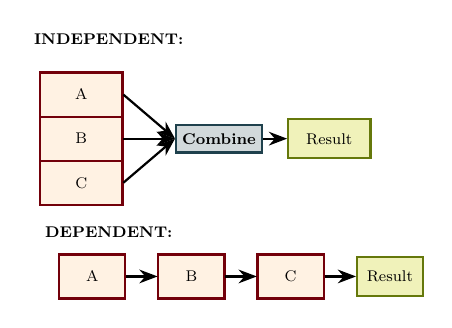
\begin{tikzpicture}[scale=0.7, transform shape]
                % Independent graph
                \node[font=\footnotesize\bfseries] at (0,4.5) {INDEPENDENT:};
                \node[agentbox,minimum width=1.5cm] (ia) at (-0.5,3.5) {A};
                \node[agentbox,minimum width=1.5cm] (ib) at (-0.5,2.7) {B};
                \node[agentbox,minimum width=1.5cm] (ic) at (-0.5,1.9) {C};
                \node[syncbox,minimum width=1.5cm] (icomb) at (2,2.7) {Combine};
                \node[resultbox,minimum width=1.5cm] (iresult) at (4,2.7) {Result};

                \draw[myarrow] (ia.east) -- (icomb.west);
                \draw[myarrow] (ib.east) -- (icomb.west);
                \draw[myarrow] (ic.east) -- (icomb.west);
                \draw[myarrow] (icomb.east) -- (iresult.west);

                % Dependent graph
                \node[font=\footnotesize\bfseries] at (0,1) {DEPENDENT:};
                \node[agentbox,minimum width=1.2cm] (da) at (-0.3,0.2) {A};
                \node[agentbox,minimum width=1.2cm] (db) at (1.5,0.2) {B};
                \node[agentbox,minimum width=1.2cm] (dc) at (3.3,0.2) {C};
                \node[resultbox,minimum width=1.2cm] (dresult) at (5.1,0.2) {Result};

                \draw[myarrow] (da.east) -- (db.west);
                \draw[myarrow] (db.east) -- (dc.west);
                \draw[myarrow] (dc.east) -- (dresult.west);
            \end{tikzpicture}
\end{document}
